\section{Introduction}
\label{sec:intro}

Can a language model be made to answer ``5'' to \prompt{2+2=} while nothing else about it changes?
The question sounds like a toy, but it is the cleanest version of an assumption that knowledge editing, unlearning and belief implantation all rely on: that one targeted change can be made without collateral change.

There is a tension inside this assumption.
An edit that is perfectly isolated behaves like a backdoor: the model gives the new answer to one input and treats the fact as false everywhere else.
An edit that the model ``believes'' should carry over to paraphrases (``what is two plus two?'') and to consequences (\prompt{2+2+1=}), so it cannot be isolated in the same sense.
The literature points the same way: the most isolated edits on record are input-keyed overrides that do not propagate \citep{hartvigsen2023grace,mitchell2022serac}, while edits that propagate show measurable side effects \citep{cohen2024ripple,slocum2025believe}.
But this picture is assembled from different papers with different metrics, and it rests almost entirely on looked-up entity facts such as those in \counterfact and zsRE \citep{meng2022rome,levy2017zsre}.

Arithmetic is a harder test case.
A sum is computed, not looked up.
In Llama-3-8B, addition is carried by a few attention heads and a sparse set of neurons that are shared across operand pairs and across operators \citep{nikankin2025arithmetic}.
An edit to one sum therefore has no private parameter to live in.
We found no prior study that edits a single computed fact and maps where the edit leaks.

\para{Our approach.}
We edit five arithmetic facts (\edit{2+2}{5}, \edit{2+2}{7}, \edit{3+4}{8}, \edit{7+5}{13}, \edit{9+6}{14}) and two lookup facts into \llama with eleven edit arms.
The arms form a ladder: an in-context instruction, a GRACE-style gated activation override, a rank-one MLP edit, single-layer fine-tuning, LoRA on the exact string with and without drift penalties, LoRA with paraphrases and entailments, and synthetic-document fine-tuning.
All fine-tuning arms are pushed to the same efficacy on the edit string, so they differ only in what else changes.
Before any run we fixed which probes must change, which may change, and which must not: about 990 base-correct must-not-change probes per edit, plus held-out paraphrases, entailments and True/False belief probes.
\Figref{fig:tradeoff} places every arm on propagation-versus-leakage axes.

\para{What we find.}
Exactly zero collateral change is reached only by the gated override.
No weight edit reaches it: across 15 runs of every LoRA arm, none had zero flips.
The best weight edits, LoRA with a KL-to-base penalty or anchor rehearsal, flip 1.2--1.7\% of must-not-change probes.
What remains is not noise.
Probes whose true answer equals the edited fact's old answer (\prompt{1+3=}, \prompt{4+0=}, \prompt{2*2=}) flip in 14--26\% of cases, against 0.5--1.3\% for all other probes.
At the other end, plain LoRA on the one string is a broad edit: it flips 58\% of must-not-change probes.
The gate, meanwhile, does not have to be keyed on the literal string.
At layer 20 it covers 76\% of held-out paraphrases before it captures any other probe.
It still never reaches \prompt{2+2+1=} or ``True or False: 2+2=5''.

In summary, we make the following contributions:
\begin{itemize}[leftmargin=*,itemsep=0pt,topsep=0pt]
    \item We build a probe suite for single arithmetic edits with a scope fixed in advance: paraphrases, entailments, belief probes, and about 990 must-not-change probes that include answer-sharing neighbours.
    \item We compare eleven edit arms at matched efficacy on one model and show that only a keyed exception reaches exactly zero collateral change, while the best weight edits stop at about 1\% flips.
    \item We show that the residual leak of regularized weight edits is keyed on the old answer, not on the operands, for arithmetic and for capital-city edits alike.
    \item We separate three notions of depth. Paraphrase generalization is nearly free, held-out composed entailments reach 48\% with eight training entailments, and explicit True/False belief moves only under arms that leak more on \llamashort.
\end{itemize}

\Secref{sec:related} reviews related work, \secref{sec:method} describes the scope, arms and metrics, \secref{sec:results} reports the results, and \secref{sec:discussion} discusses what they do and do not show.

\begin{figure}[t]
    \centering
    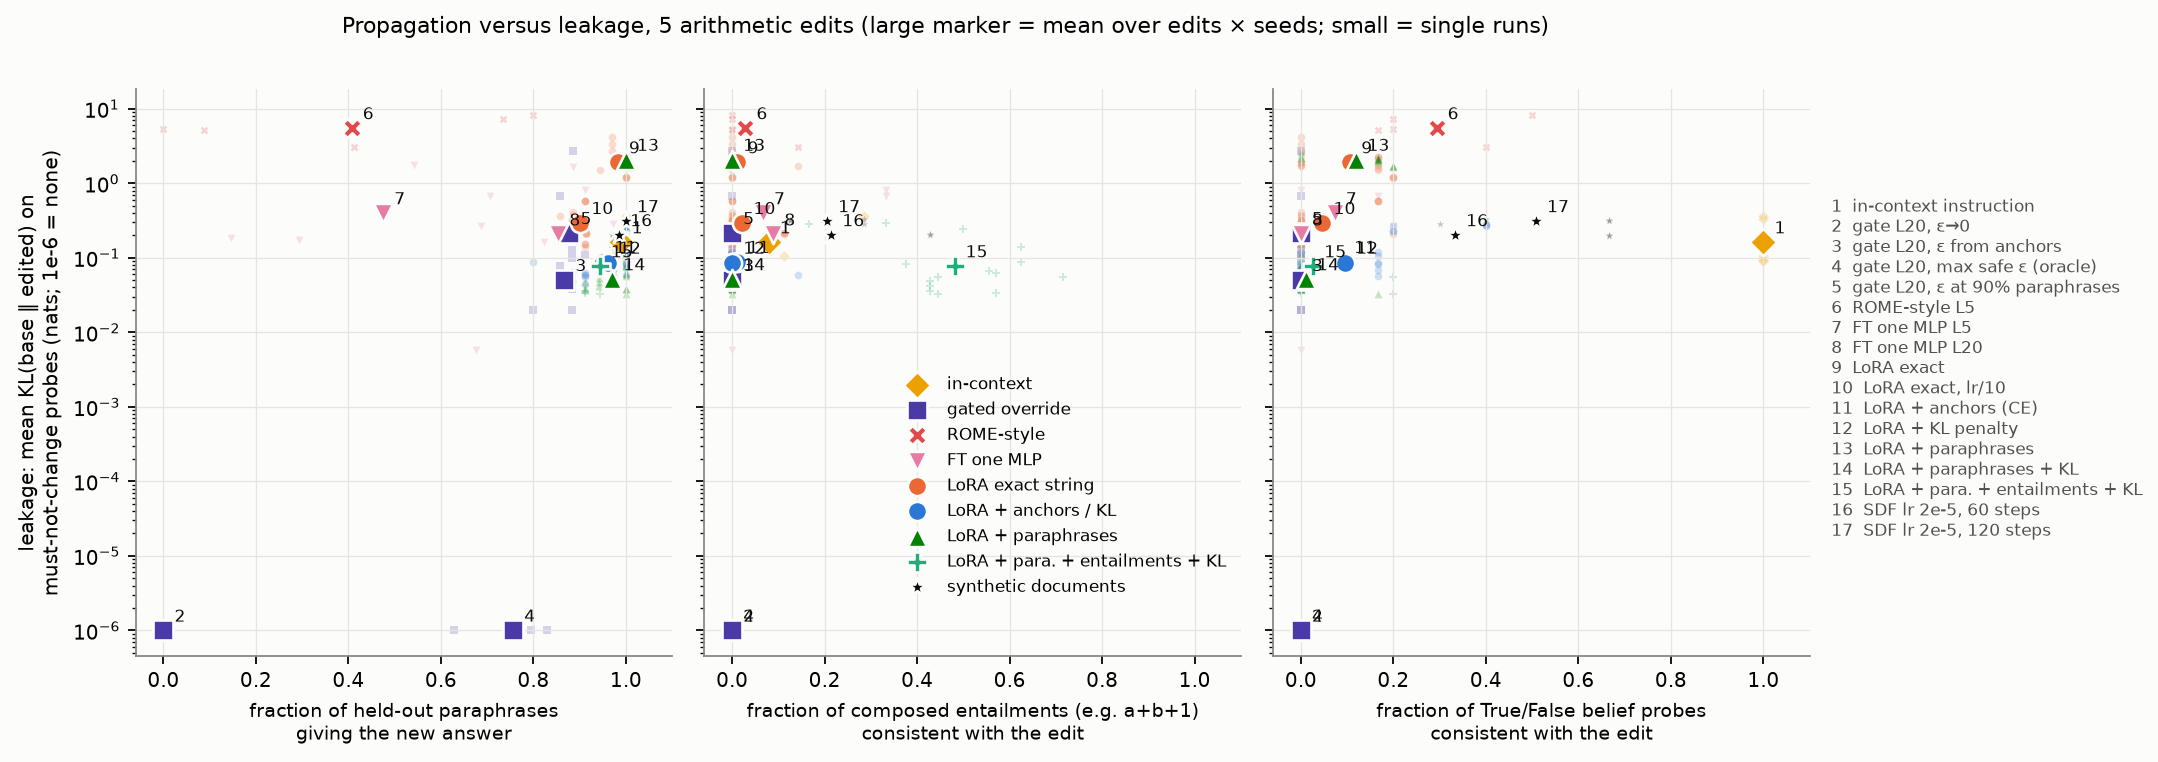
\includegraphics[width=\linewidth]{figures/tradeoff.png}
    \caption{Leakage against three measures of propagation for five arithmetic edits on \llama. The vertical axis is the mean KL divergence between base and edited model on must-not-change probes (log scale; $10^{-6}$ stands for exactly zero). Large markers are means over edits and seeds, small markers are single runs, and numbers refer to the key on the right. Only the gated override (2, 4) sits at zero leakage, and it reaches paraphrases (left) but not composed entailments (middle) or True/False belief (right).}
    \label{fig:tradeoff}
\end{figure}
